% Slide 1
\begin{frame}
  \frametitle{Optical Flow}
  \note{https://docs.opencv.org/3.4/d4/dee/tutorial_optical_flow.html}
  \note{https://youtu.be/lnXFcmLB7sM}
  \note{https://www.baeldung.com/cs/motion-field-optical-flow}
  \note{https://rpg.ifi.uzh.ch/docs/teaching/2020/11_tracking.pdf}
  \note{https://rpg.ifi.uzh.ch/teaching.html\#VAMR}
  \note{https://asl.ethz.ch/education/lectures/autonomous_mobile_robots/spring-2021.html}
  \note{https://cs.brown.edu/courses/cs143/2011/results/proj5/gen/}
  \note{https://rpg.ifi.uzh.ch/docs/teaching/2025/03_camera_calibration.pdf}

    Method to estimate apparent motion of scene points from a sequence of images.

    Optical flow is the pattern of apparent motion of image objects between two consecutive frames caused by the movement of object or camera. It is 2D vector field where each vector is a displacement vector showing the movement of points from first frame to second.

    \begin{columns}
      \begin{column}{0.5\textwidth}
        \begin{center}
          \movie[showcontrols,autostart,loop,poster]{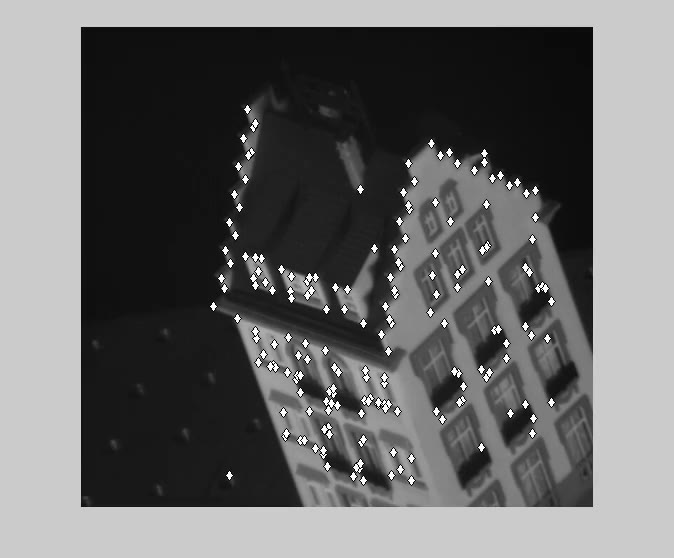
\includegraphics[width=0.8\columnwidth]{images/optical_flow/klt_points_video.jpg}}{videos/klt_points.mp4}
        \end{center}
      \end{column}
      \begin{column}{0.5\textwidth}  %%<--- here
        \begin{center}
          \movie[showcontrols,autostart,loop,poster]{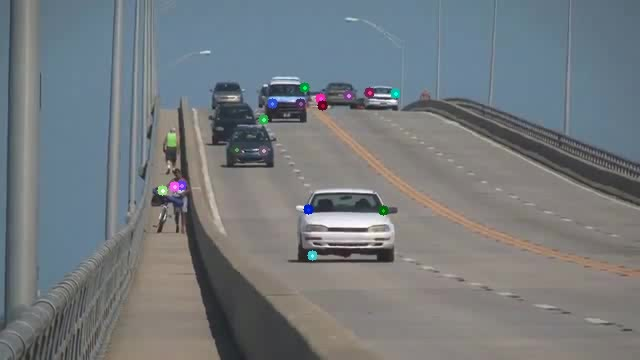
\includegraphics[width=\columnwidth]{images/optical_flow/klt_tracking_video.jpg}}{videos/klt_tracking.mp4}
        \end{center}
      \end{column}
    \end{columns}

    Topics:
    \begin{enumerate}
    \item Motion Field and Optical Flow
    \item Optical Flow Constraint Equation
    \item Lucas-Kanade Method
    \item Coarse-to-Fine Flow Estimation
    \item Applications of Optical Flow
    \end{enumerate}
\end{frame}

% Slide 2
\begin{frame}
  \frametitle{Motion Field and Optical Flow}
    Consider a point in the 3D scene which is moving in some direction. The projection of that motion onto the 2D image plane is referred to as the motion field. Unfortunately, there is no guarantee that we can measure this motion field; all we can measure is the motion of brightness patterns, referred to as the optical flow.

    \vspace{0.5cm}
    \centering
    % \includegraphics[width=0.6\textwidth]{placeholder-slide3.png}
\end{frame}

% Slide 3
\begin{frame}
  \frametitle{Optical Flow}
Motion of brightness patterns in the image.

Ideally: Optical Flow = Motion Field.

\vspace{0.5cm}
\centering
% \includegraphics[width=0.6\textwidth]{placeholder-slide6.png}
\end{frame}

% Slide 4
\begin{frame}
  \frametitle{When is Optical Flow $\neq$ Motion Field?}
\begin{itemize}
  \item Motion Field exists but no Optical Flow (e.g., spinning sphere, stationary light source)
  \item No Motion Field exists but there is Optical Flow (e.g., stationary sphere, moving light source)
\end{itemize}

\vspace{0.5cm}
\centering
% \includegraphics[width=0.6\textwidth]{placeholder-slide7.png}
\end{frame}

% Slide 5
\begin{frame}
  \frametitle{Motion Illusions}
\begin{itemize}
  \item Barber Pole Illusion: Motion Field horizontal, Optical Flow appears vertical.
  \item Donguri Wave Illusion: Static image but perceived motion.
  \item Ouchi Pattern: Inner disc appears to move with respect to the ring.
\end{itemize}

\vspace{0.5cm}
\centering
% \includegraphics[width=0.6\textwidth]{placeholder-slide9.png}
\end{frame}

% Slide 6
\begin{frame}
  \frametitle{Optical Flow Constraint Equation}
\textbf{Assumption 1:} Brightness of image point remains constant over time.

$ I(x,y,t) = I(x+\delta x, y+\delta y, t+\delta t) $

\vspace{0.5cm}
\centering
% \includegraphics[width=0.6\textwidth]{placeholder-slide13.png}
\end{frame}

% Slide 7
\begin{frame}
  \frametitle{Optical Flow Constraint Equation}
\textbf{Assumption 2:} Displacements ($\delta x, \delta y$) and time step $\delta t$ are small.

Taylor expansion approximation:

$ I(x+\delta x, y+\delta y, t+\delta t) \approx I(x,y,t) + I_x \delta x + I_y \delta y + I_t \delta t $

\end{frame}

% Slide 8
\begin{frame}
  \frametitle{Constraint Equation}
After simplification:

$ I_x u + I_y v + I_t = 0 $

This is the \textbf{Optical Flow Constraint Equation}.

\vspace{0.5cm}
\centering
% \includegraphics[width=0.6\textwidth]{placeholder-slide17.png}
\end{frame}

% Slide 9
\begin{frame}
  \frametitle{Normal Flow and Aperture Problem}
\begin{itemize}
  \item Constraint equation gives only a line in $(u,v)$ space.
  \item Can compute normal flow but not full optical flow.
  \item Locally, humans also perceive only normal flow (aperture problem).
\end{itemize}

\vspace{0.5cm}
\centering
% \includegraphics[width=0.6\textwidth]{placeholder-slide22.png}
\end{frame}

% Slide 10
\begin{frame}
  \frametitle{Lucas-Kanade Method}
\textbf{Assumption:} Optical flow is constant in a small neighborhood.

Formulate system of equations and solve using least squares.

\vspace{0.5cm}
\centering
% \includegraphics[width=0.6\textwidth]{placeholder-slide25.png}
\end{frame}

% Slide 11
\begin{frame}
  \frametitle{When Does Optical Flow Estimation Work?}
\begin{itemize}
  \item Smooth regions: Bad (small eigenvalues).
  \item Edges: Bad (aperture problem).
  \item Textured regions: Good (large, diverse gradients).
\end{itemize}

\vspace{0.5cm}
\centering
% \includegraphics[width=0.6\textwidth]{placeholder-slide32.png}
\end{frame}

% Slide 12
\begin{frame}
  \frametitle{Large Motion: Problem}
Taylor approximation invalid when displacements are large.

\vspace{0.5cm}
\centering
% \includegraphics[width=0.6\textwidth]{placeholder-slide34.png}
\end{frame}

% Slide 13
\begin{frame}
  \frametitle{Coarse-to-Fine Estimation}
Use resolution pyramid:
\begin{itemize}
  \item Compute flow at low resolution.
  \item Warp and refine at higher resolutions.
  \item Repeat until full resolution.
\end{itemize}

\vspace{0.5cm}
\centering
% \includegraphics[width=0.6\textwidth]{placeholder-slide36.png}
\end{frame}

% Slide 14
\begin{frame}
  \frametitle{Alternative Approach: Template Matching}
\begin{itemize}
  \item Use template window from one frame.
  \item Search for best match in next frame.
  \item Difference gives optical flow.
  \item Slow and can produce mismatches.
\end{itemize}

\vspace{0.5cm}
\centering
% \includegraphics[width=0.6\textwidth]{placeholder-slide41.png}
\end{frame}

% Slide 15
\begin{frame}
  \frametitle{Applications of Optical Flow}
\begin{itemize}
  \item Optical mouse: motion tracking.
  \item Traffic monitoring: estimate vehicle speed.
  \item Video retiming: slow motion.
  \item Stabilization: remove camera shake.
  \item Face tracking: expressions, blinking.
\end{itemize}

\vspace{0.5cm}
\centering
% \includegraphics[width=0.6\textwidth]{placeholder-slide47.png}
\end{frame}

% References
% \begin{frame}
%   \frametitle{References}
%     \tiny
%     [Barron 2005] J. L. Barron, D. J. Fleet, and S. Beauchemin, IJCV 2005. \\
%     [Black 1993] M. J. Black and P. Anandan, ICCV 1993. \\
%     [Bouguet 2000] J. Y. Bouguet, Intel Tech Report 2000. \\
%     [Brox 2004] T. Brox, A. Bruhn, N. Papenberg, J. Weickert, ECCV 2004. \\
%     [Horn 1981] B. K. P. Horn and B. G. Schunck, AI 1981. \\
%     [Liu 2014] S. Liu, L. Yuan, P. Tan, J. Sun, CVPR 2014. \\
%     [Lucas 1981] B. D. Lucas and T. Kanade, Imaging Workshop 1981.
% \end{frame}